\documentclass{ximera}
\input{../preamble.tex}

\author{Robert Kenney \and Paul Zachlin \and Nicholas Shay}
\title{An Application of X-bar Charts to Manufacturing} \license{CC BY-NC-SA 4.0}
\begin{document}

\begin{abstract}
We study basic ideas behind the use of control charts in industry.
\end{abstract}
\maketitle

\begin{onlineOnly}
\section*{An Application of X-bar Charts to Manufacturing}
\end{onlineOnly}

In \emph{thermoform production}, plastic sheets are fed into machines which can turn them into molded plastic objects which are used in everyday life.  As an example, consider the molded plastic container holding the ``surprise" inside of the chocolate candy in the picture below.

\begin{center}
        \begin{tikzpicture}
\node[inner sep=0pt, anchor=base] (p1) at (0,0)
  {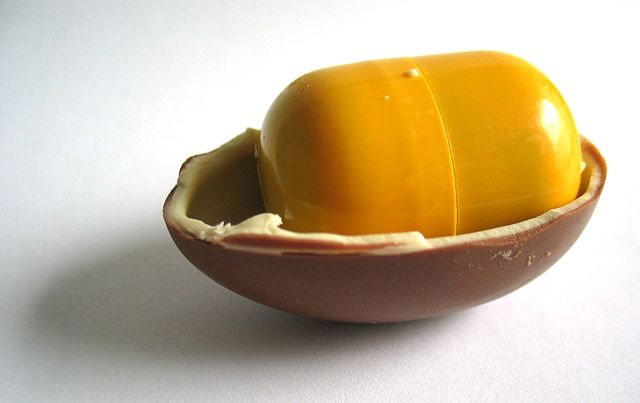
\includegraphics[height=60mm]{Kinder_Surprise.jpg}};
           \end{tikzpicture}
      \end{center}

In the following Desmos graph we can view 16 samples of 5 diameters measured during thermoform production in Taiwan.  From prior production runs it was known that the mean diameter was $\mu = 34.75$ mm, and the standard deviation was $\sigma = 0.17$ mm.  Let's assume that the samples are taken every hour.  For the ``surprise" to fit inside the plastic shell, and for the plastic shell to fit inside the chocolate candy, specification limits are set to $34.75\pm 0.55$ mm.  Any thermoform with a diameter greater than 35.3 mm or less than 34.2 mm is unusable.
 
\desmos{uxhaiyqoso}{800}{600}

We can see that after the first 12 hours of production, most of the diameters that were sampled were too big, and so many thermoforms had to be scrapped.  The point of Statistical Process Control is to detect signs of a process being out of control, so that corrections can be made and waste can be reduced.  Were there signs that this thermoform production process was out of control earlier?  In this section we will see how control charts can be used to detect an out of control process before scrap is produced.  

\subsection*{When is it time to investigate?}

There will always be some variation in any process.  %At this point you have studied enough statistics to know that a very important idea is to determine when variation is \emph{significant} (i.e. worthy of further investigation).
One of the fundamental principles of statistical process control is that if a process is acting in a non-random way, the process can be improved.  Control charts are used to detect non-random behavior. In the previous section we discussed several general trends seen in control charts that indicate an out-of-control process.  We now formalize our previous observations with a set of rules.  The
 \href{https://www.qimacros.com/control-chart/nelson-rules/}{Nelson rules} for control charts is a common set of rules used in manufacturing to determine when a process may be out-of-control.  %We consider any of the following eight scenarios to be significant. 

 Recall, from the previous section, that control limits are typically set at three standard deviations away from the mean, where standard deviation, $\sigma_{\bar{X}}$ is given by the Central Limit Theorem to be 
 $$\sigma_{\bar{X}}=\frac{\sigma}{\sqrt{n}}$$
 where $\sigma$ is population standard deviation and $n$ is the sample size.

 
\begin{definition}[Nelson Rules]\label{def:nelson}
\textbf{Rule 1:}  One point falls above UCL or below LCL.

\begin{center}
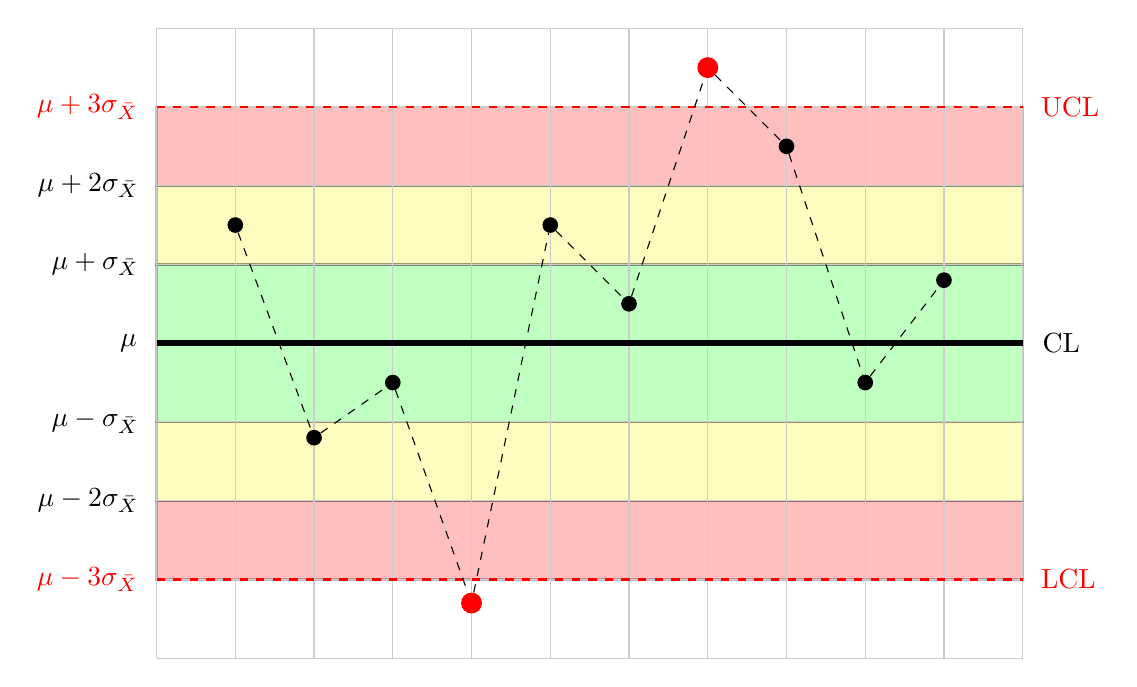
\begin{tikzpicture}[scale=1]
\draw[black, thick, fill=green,opacity=0.25] (0,-1) rectangle (11, 1);
\draw[black, thick, fill=yellow,opacity=0.25] (0,-2) rectangle (11, -1);
\draw[black, thick, fill=yellow,opacity=0.25] (0,1) rectangle (11, 2);
\draw[black, thick, fill=red,opacity=0.25] (0,-3) rectangle (11, -2);
\draw[black, thick, fill=red,opacity=0.25] (0,2) rectangle (11, 3);
\draw[thin,gray!40] (0,-4) grid (11,4);
\draw[line width=2pt](0,0)node[left=1mm]{$\mu$}--(11,0)node[right=1mm]{CL} ;
 \draw[line width=1pt,red, dashed](0,3)node[left=1mm]{$\mu+3\sigma_{\bar{X}}$}--(11,3)node[right=1mm]{UCL};
\draw[line width=1pt,red, dashed](0,-3)node[left=1mm]{$\mu-3\sigma_{\bar{X}}$}--(11,-3)node[right=1mm]{LCL};

\node[left=1mm] at (0,1){$\mu+\sigma_{\bar{X}}$};
\node[left=1mm] at (0,-1){$\mu-\sigma_{\bar{X}}$};
\node[left=1mm] at (0,2){$\mu+2\sigma_{\bar{X}}$};
\node[left=1mm] at (0,-2){$\mu-2\sigma_{\bar{X}}$};

 \node (A) at (1,1.5) [circle,fill=black,scale=0.6]{};
 \node (B) at (2,-1.2) [circle,fill=black,scale=0.6]{};
 \node (C) at (3,-0.5) [circle,fill=black,scale=0.6]{};
 \node (D) at (4,-3.3) [circle,fill=red,scale=0.8]{};
 \node (E) at (5,1.5) [circle,fill=black,scale=0.6]{};
 \node (F) at (6,0.5) [circle,fill=black,scale=0.6]{};
\node (G) at (7,3.5) [circle,fill=red,scale=0.8]{};
\node (H) at (8,2.5) [circle,fill=black,scale=0.6]{};
\node (I) at (9,-0.5) [circle,fill=black,scale=0.6]{};
\node (J) at (10,0.8) [circle,fill=black,scale=0.6]{};

\draw[-,dashed] (A)--(B); 
\draw[-,dashed] (B)--(C);
\draw[-,dashed] (C)--(D);
\draw[-,dashed] (D)--(E); 
\draw[-,dashed] (E)--(F);
\draw[-,dashed] (F)--(G); 
\draw[-,dashed] (G)--(H);
\draw[-,dashed] (H)--(I);
\draw[-,dashed] (I)--(J);

 \end{tikzpicture}
\end{center}

\textbf{Rule 2:}  Two out of three consecutive points are on the same side of the center line and above $\mu+2\sigma_{\bar{X}}$ or below $\mu-2\sigma_{\bar{X}}$.

\begin{center}
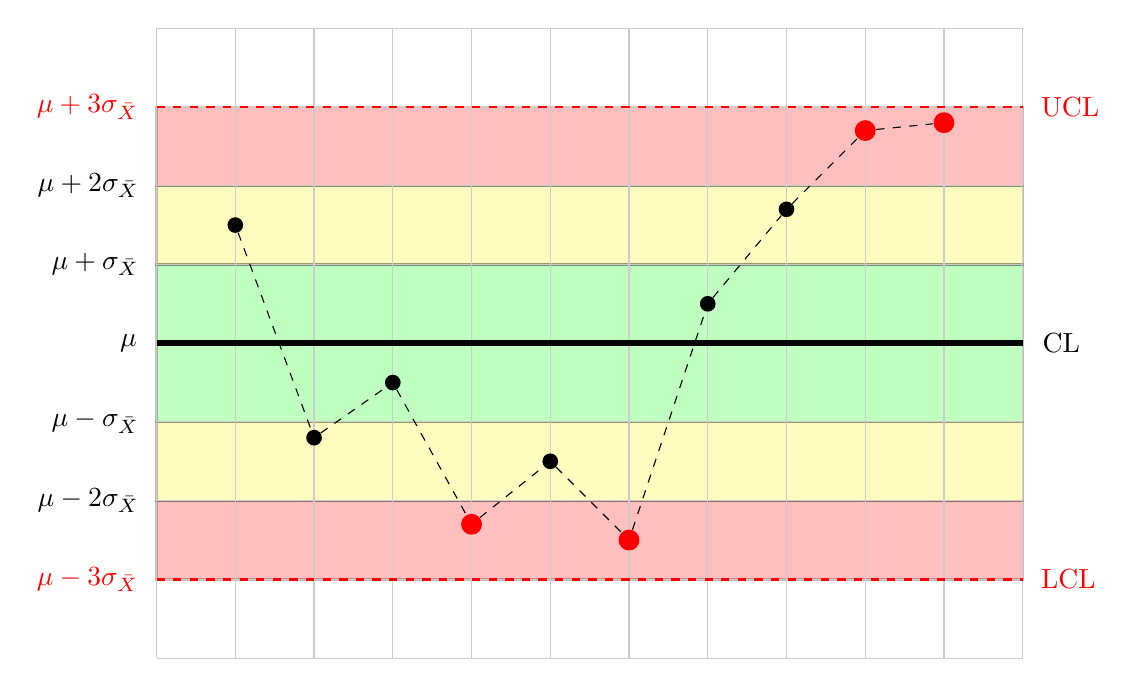
\begin{tikzpicture}[scale=1]
\draw[black, thick, fill=green,opacity=0.25] (0,-1) rectangle (11, 1);
\draw[black, thick, fill=yellow,opacity=0.25] (0,-2) rectangle (11, -1);
\draw[black, thick, fill=yellow,opacity=0.25] (0,1) rectangle (11, 2);
\draw[black, thick, fill=red,opacity=0.25] (0,-3) rectangle (11, -2);
\draw[black, thick, fill=red,opacity=0.25] (0,2) rectangle (11, 3);
\draw[thin,gray!40] (0,-4) grid (11,4);
\draw[line width=2pt](0,0)node[left=1mm]{$\mu$}--(11,0)node[right=1mm]{CL} ;
 \draw[line width=1pt,red, dashed](0,3)node[left=1mm]{$\mu+3\sigma_{\bar{X}}$}--(11,3)node[right=1mm]{UCL};
\draw[line width=1pt,red, dashed](0,-3)node[left=1mm]{$\mu-3\sigma_{\bar{X}}$}--(11,-3)node[right=1mm]{LCL};

\node[left=1mm] at (0,1){$\mu+\sigma_{\bar{X}}$};
\node[left=1mm] at (0,-1){$\mu-\sigma_{\bar{X}}$};
\node[left=1mm] at (0,2){$\mu+2\sigma_{\bar{X}}$};
\node[left=1mm] at (0,-2){$\mu-2\sigma_{\bar{X}}$};

 \node (A) at (1,1.5) [circle,fill=black,scale=0.6]{};
 \node (B) at (2,-1.2) [circle,fill=black,scale=0.6]{};
 \node (C) at (3,-0.5) [circle,fill=black,scale=0.6]{};
 \node (D) at (4,-2.3) [circle,fill=red,scale=0.8]{};
 \node (E) at (5,-1.5) [circle,fill=black,scale=0.6]{};
 \node (F) at (6,-2.5) [circle,fill=red,scale=0.8]{};
\node (G) at (7,0.5) [circle,fill=black,scale=0.6]{};
\node (H) at (8,1.7) [circle,fill=black,scale=0.6]{};
\node (I) at (9,2.7) [circle,fill=red,scale=0.8]{};
\node (J) at (10,2.8) [circle,fill=red,scale=0.8]{};

\draw[-,dashed] (A)--(B); 
\draw[-,dashed] (B)--(C);
\draw[-,dashed] (C)--(D);
\draw[-,dashed] (D)--(E); 
\draw[-,dashed] (E)--(F);
\draw[-,dashed] (F)--(G); 
\draw[-,dashed] (G)--(H);
\draw[-,dashed] (H)--(I);
\draw[-,dashed] (I)--(J);

 \end{tikzpicture}
\end{center}

\textbf{Rule 3:} Four out of five consecutive points are on the same side of the center line and above $\mu+\sigma_{\bar{X}}$ or below $\mu-\sigma_{\bar{X}}$.

\begin{center}
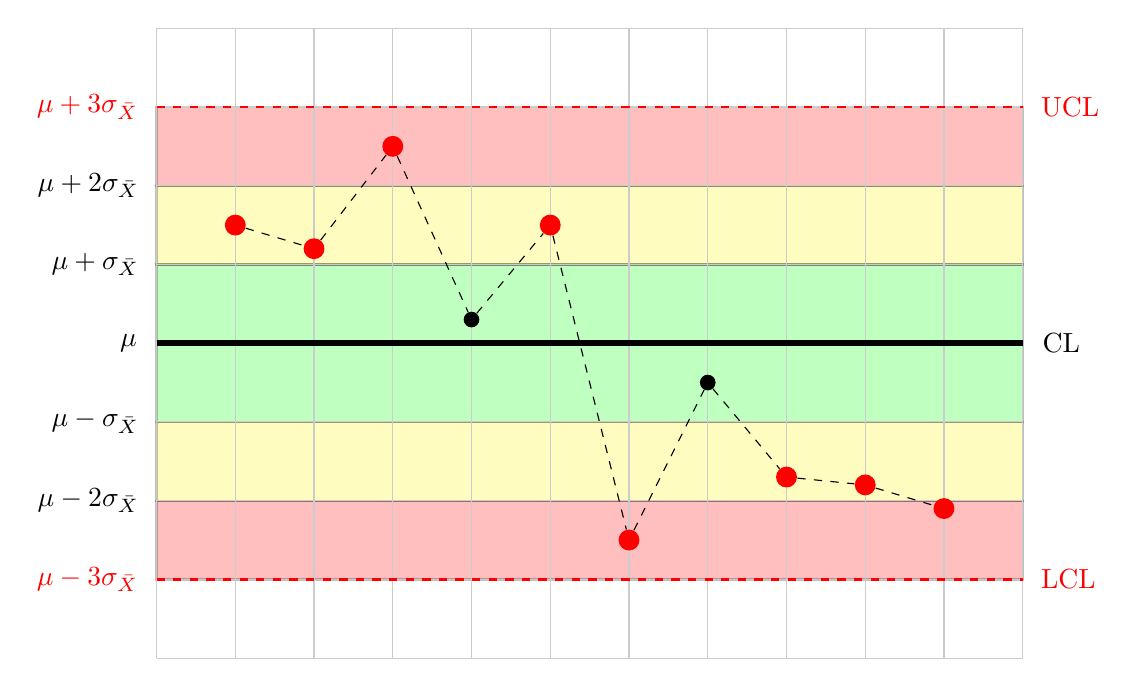
\begin{tikzpicture}[scale=1]
\draw[black, thick, fill=green,opacity=0.25] (0,-1) rectangle (11, 1);
\draw[black, thick, fill=yellow,opacity=0.25] (0,-2) rectangle (11, -1);
\draw[black, thick, fill=yellow,opacity=0.25] (0,1) rectangle (11, 2);
\draw[black, thick, fill=red,opacity=0.25] (0,-3) rectangle (11, -2);
\draw[black, thick, fill=red,opacity=0.25] (0,2) rectangle (11, 3);
\draw[thin,gray!40] (0,-4) grid (11,4);
\draw[line width=2pt](0,0)node[left=1mm]{$\mu$}--(11,0)node[right=1mm]{CL} ;
 \draw[line width=1pt,red, dashed](0,3)node[left=1mm]{$\mu+3\sigma_{\bar{X}}$}--(11,3)node[right=1mm]{UCL};
\draw[line width=1pt,red, dashed](0,-3)node[left=1mm]{$\mu-3\sigma_{\bar{X}}$}--(11,-3)node[right=1mm]{LCL};

\node[left=1mm] at (0,1){$\mu+\sigma_{\bar{X}}$};
\node[left=1mm] at (0,-1){$\mu-\sigma_{\bar{X}}$};
\node[left=1mm] at (0,2){$\mu+2\sigma_{\bar{X}}$};
\node[left=1mm] at (0,-2){$\mu-2\sigma_{\bar{X}}$};

 \node (A) at (1,1.5) [circle,fill=red,scale=0.8]{};
 \node (B) at (2,1.2) [circle,fill=red,scale=0.8]{};
 \node (C) at (3,2.5) [circle,fill=red,scale=0.8]{};
 \node (D) at (4,0.3) [circle,fill=black,scale=0.6]{};
 \node (E) at (5,1.5) [circle,fill=red,scale=0.8]{};
 \node (F) at (6,-2.5) [circle,fill=red,scale=0.8]{};
\node (G) at (7,-0.5) [circle,fill=black,scale=0.6]{};
\node (H) at (8,-1.7) [circle,fill=red,scale=0.8]{};
\node (I) at (9,-1.8) [circle,fill=red,scale=0.8]{};
\node (J) at (10,-2.1) [circle,fill=red,scale=0.8]{};

\draw[-,dashed] (A)--(B); 
\draw[-,dashed] (B)--(C);
\draw[-,dashed] (C)--(D);
\draw[-,dashed] (D)--(E); 
\draw[-,dashed] (E)--(F);
\draw[-,dashed] (F)--(G); 
\draw[-,dashed] (G)--(H);
\draw[-,dashed] (H)--(I);
\draw[-,dashed] (I)--(J);

 \end{tikzpicture}
\end{center}

\textbf{Rule 4:} Eight consecutive points are on the same side of the center line.

\begin{center}
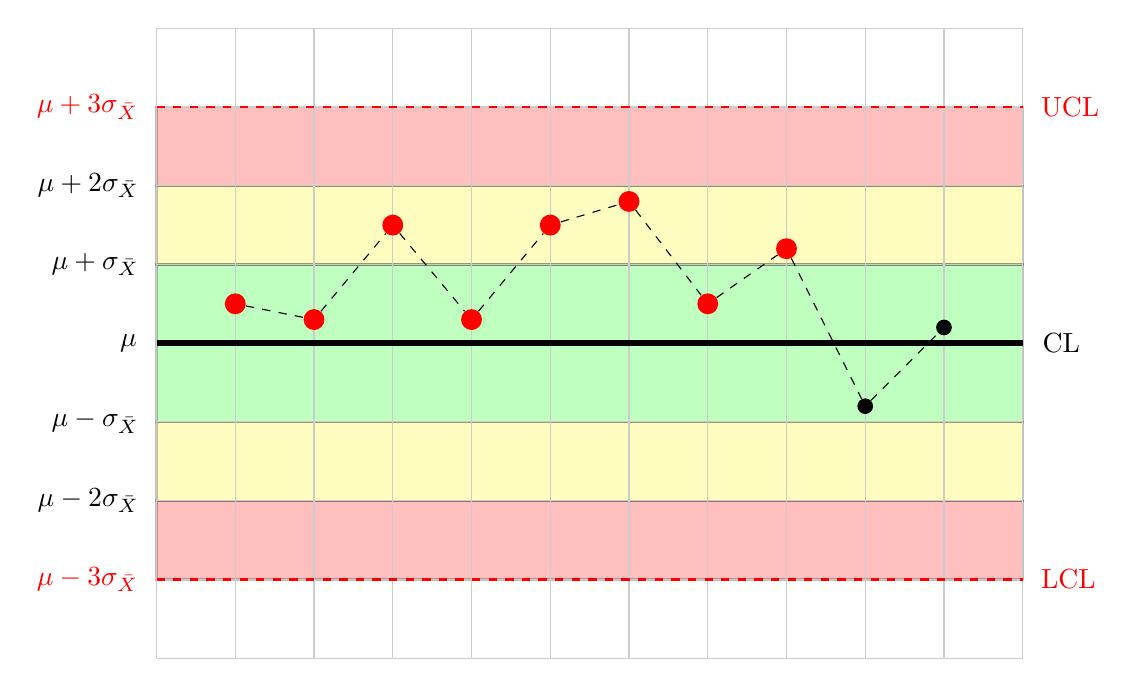
\begin{tikzpicture}[scale=1]
\draw[black, thick, fill=green,opacity=0.25] (0,-1) rectangle (11, 1);
\draw[black, thick, fill=yellow,opacity=0.25] (0,-2) rectangle (11, -1);
\draw[black, thick, fill=yellow,opacity=0.25] (0,1) rectangle (11, 2);
\draw[black, thick, fill=red,opacity=0.25] (0,-3) rectangle (11, -2);
\draw[black, thick, fill=red,opacity=0.25] (0,2) rectangle (11, 3);
\draw[thin,gray!40] (0,-4) grid (11,4);
\draw[line width=2pt](0,0)node[left=1mm]{$\mu$}--(11,0)node[right=1mm]{CL} ;
 \draw[line width=1pt,red, dashed](0,3)node[left=1mm]{$\mu+3\sigma_{\bar{X}}$}--(11,3)node[right=1mm]{UCL};
\draw[line width=1pt,red, dashed](0,-3)node[left=1mm]{$\mu-3\sigma_{\bar{X}}$}--(11,-3)node[right=1mm]{LCL};

\node[left=1mm] at (0,1){$\mu+\sigma_{\bar{X}}$};
\node[left=1mm] at (0,-1){$\mu-\sigma_{\bar{X}}$};
\node[left=1mm] at (0,2){$\mu+2\sigma_{\bar{X}}$};
\node[left=1mm] at (0,-2){$\mu-2\sigma_{\bar{X}}$};

 \node (A) at (1,0.5) [circle,fill=red,scale=0.8]{};
 \node (B) at (2,0.3) [circle,fill=red,scale=0.8]{};
 \node (C) at (3,1.5) [circle,fill=red,scale=0.8]{};
 \node (D) at (4,0.3) [circle,fill=red,scale=0.8]{};
 \node (E) at (5,1.5) [circle,fill=red,scale=0.8]{};
 \node (F) at (6,1.8) [circle,fill=red,scale=0.8]{};
\node (G) at (7,0.5) [circle,fill=red,scale=0.8]{};
\node (H) at (8,1.2) [circle,fill=red,scale=0.8]{};
\node (I) at (9,-0.8) [circle,fill=black,scale=0.6]{};
\node (J) at (10,0.2) [circle,fill=black,scale=0.6]{};

\draw[-,dashed] (A)--(B); 
\draw[-,dashed] (B)--(C);
\draw[-,dashed] (C)--(D);
\draw[-,dashed] (D)--(E); 
\draw[-,dashed] (E)--(F);
\draw[-,dashed] (F)--(G); 
\draw[-,dashed] (G)--(H);
\draw[-,dashed] (H)--(I);
\draw[-,dashed] (I)--(J);

 \end{tikzpicture}
\end{center}

\textbf{Rule 5:} Six consecutive points are ascending/decending. 

\begin{center}
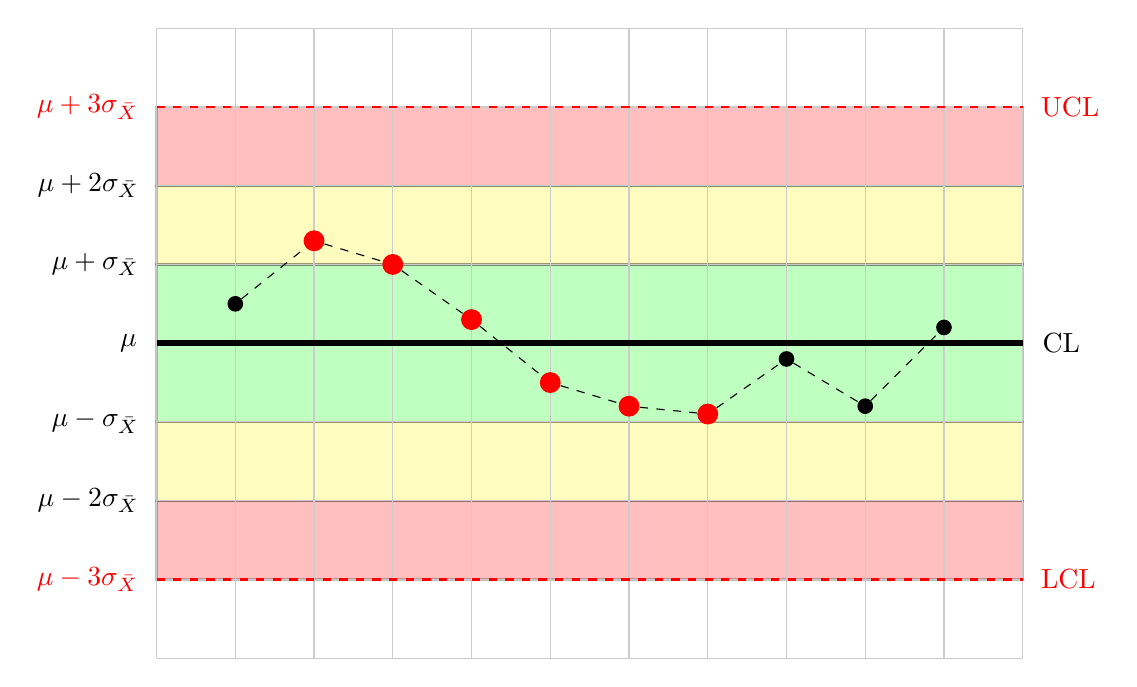
\begin{tikzpicture}[scale=1]
\draw[black, thick, fill=green,opacity=0.25] (0,-1) rectangle (11, 1);
\draw[black, thick, fill=yellow,opacity=0.25] (0,-2) rectangle (11, -1);
\draw[black, thick, fill=yellow,opacity=0.25] (0,1) rectangle (11, 2);
\draw[black, thick, fill=red,opacity=0.25] (0,-3) rectangle (11, -2);
\draw[black, thick, fill=red,opacity=0.25] (0,2) rectangle (11, 3);
\draw[thin,gray!40] (0,-4) grid (11,4);
\draw[line width=2pt](0,0)node[left=1mm]{$\mu$}--(11,0)node[right=1mm]{CL} ;
 \draw[line width=1pt,red, dashed](0,3)node[left=1mm]{$\mu+3\sigma_{\bar{X}}$}--(11,3)node[right=1mm]{UCL};
\draw[line width=1pt,red, dashed](0,-3)node[left=1mm]{$\mu-3\sigma_{\bar{X}}$}--(11,-3)node[right=1mm]{LCL};

\node[left=1mm] at (0,1){$\mu+\sigma_{\bar{X}}$};
\node[left=1mm] at (0,-1){$\mu-\sigma_{\bar{X}}$};
\node[left=1mm] at (0,2){$\mu+2\sigma_{\bar{X}}$};
\node[left=1mm] at (0,-2){$\mu-2\sigma_{\bar{X}}$};

 \node (A) at (1,0.5) [circle,fill=black,scale=0.6]{};
 \node (B) at (2,1.3) [circle,fill=red,scale=0.8]{};
 \node (C) at (3,1) [circle,fill=red,scale=0.8]{};
 \node (D) at (4,0.3) [circle,fill=red,scale=0.8]{};
 \node (E) at (5,-0.5) [circle,fill=red,scale=0.8]{};
 \node (F) at (6,-0.8) [circle,fill=red,scale=0.8]{};
\node (G) at (7,-0.9) [circle,fill=red,scale=0.8]{};
\node (H) at (8,-0.2) [circle,fill=black,scale=0.6]{};
\node (I) at (9,-0.8) [circle,fill=black,scale=0.6]{};
\node (J) at (10,0.2) [circle,fill=black,scale=0.6]{};

\draw[-,dashed] (A)--(B); 
\draw[-,dashed] (B)--(C);
\draw[-,dashed] (C)--(D);
\draw[-,dashed] (D)--(E); 
\draw[-,dashed] (E)--(F);
\draw[-,dashed] (F)--(G); 
\draw[-,dashed] (G)--(H);
\draw[-,dashed] (H)--(I);
\draw[-,dashed] (I)--(J);

 \end{tikzpicture}
\end{center}

\textbf{Rule 6:} Fifteen consecutive points are between $\mu-\sigma_{\bar{X}}$ and $\mu+\sigma_{\bar{X}}$.  This is known as ``hugging the center line".

\textbf{Rule 7:} Fourteen consecutive points form an alternating up/down pattern.

\textbf{Rule 8:}  Eight consecutive points are above $\mu+\sigma_{\bar{X}}$ or below $\mu-\sigma_{\bar{X}}$.

\begin{center}
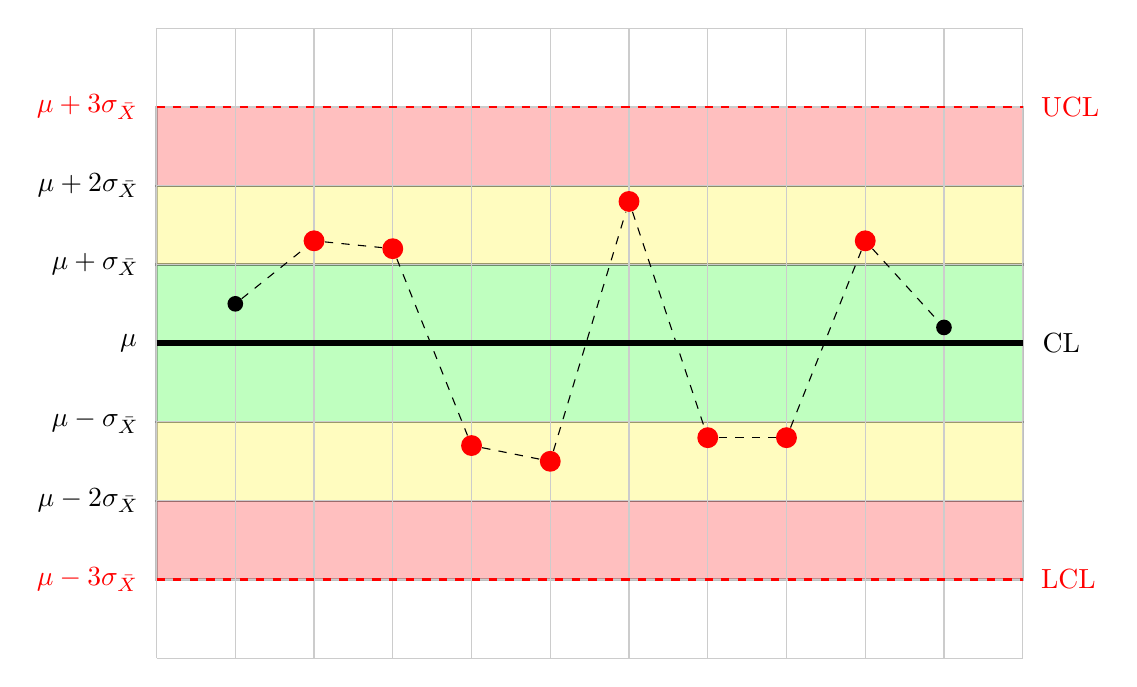
\begin{tikzpicture}[scale=1]
\draw[black, thick, fill=green,opacity=0.25] (0,-1) rectangle (11, 1);
\draw[black, thick, fill=yellow,opacity=0.25] (0,-2) rectangle (11, -1);
\draw[black, thick, fill=yellow,opacity=0.25] (0,1) rectangle (11, 2);
\draw[black, thick, fill=red,opacity=0.25] (0,-3) rectangle (11, -2);
\draw[black, thick, fill=red,opacity=0.25] (0,2) rectangle (11, 3);
\draw[thin,gray!40] (0,-4) grid (11,4);
\draw[line width=2pt](0,0)node[left=1mm]{$\mu$}--(11,0)node[right=1mm]{CL} ;
 \draw[line width=1pt,red, dashed](0,3)node[left=1mm]{$\mu+3\sigma_{\bar{X}}$}--(11,3)node[right=1mm]{UCL};
\draw[line width=1pt,red, dashed](0,-3)node[left=1mm]{$\mu-3\sigma_{\bar{X}}$}--(11,-3)node[right=1mm]{LCL};

\node[left=1mm] at (0,1){$\mu+\sigma_{\bar{X}}$};
\node[left=1mm] at (0,-1){$\mu-\sigma_{\bar{X}}$};
\node[left=1mm] at (0,2){$\mu+2\sigma_{\bar{X}}$};
\node[left=1mm] at (0,-2){$\mu-2\sigma_{\bar{X}}$};

 \node (A) at (1,0.5) [circle,fill=black,scale=0.6]{};
 \node (B) at (2,1.3) [circle,fill=red,scale=0.8]{};
 \node (C) at (3,1.2) [circle,fill=red,scale=0.8]{};
 \node (D) at (4,-1.3) [circle,fill=red,scale=0.8]{};
 \node (E) at (5,-1.5) [circle,fill=red,scale=0.8]{};
 \node (F) at (6,1.8) [circle,fill=red,scale=0.8]{};
\node (G) at (7,-1.2) [circle,fill=red,scale=0.8]{};
\node (H) at (8,-1.2) [circle,fill=red,scale=0.8]{};
\node (I) at (9,1.3) [circle,fill=red,scale=0.8]{};
\node (J) at (10,0.2) [circle,fill=black,scale=0.6]{};

\draw[-,dashed] (A)--(B); 
\draw[-,dashed] (B)--(C);
\draw[-,dashed] (C)--(D);
\draw[-,dashed] (D)--(E); 
\draw[-,dashed] (E)--(F);
\draw[-,dashed] (F)--(G); 
\draw[-,dashed] (G)--(H);
\draw[-,dashed] (H)--(I);
\draw[-,dashed] (I)--(J);

 \end{tikzpicture}
\end{center}
\end{definition}
See if you can apply the Nelson rules in the following problem.

\begin{problem}\label{prob:controlChartWithSlider}
Suppose that a manufacturing process is known to have a normal distribution with a mean $\mu=3.5$, and standard deviation $\sigma=2$.  A random sample of size $n=4$ is collected every hour to monitor the manufacturing process.  The distribution of sample means (sampling distribution) will be normal and $$\mu_{\bar{x}}=\answer{3.5},\quad \sigma_{\bar{x}}=\answer{1}$$

Determine upper and lower control limits ($\pm 3\sigma$), for the $\bar{X}$-control chart for this manufacturing process.

$$LCL=\answer{0.5},\quad UCL=\answer{6.5}$$

The GeoGebra interactive below shows the means of consecutive samples $1$ through $32$ taken over the course of two days.  Use the scroll bar to navigate all samples and answer the questions below.

\begin{onlineOnly}
\begin{center}
\geogebra{jeu5trsd}{950}{650}
\end{center}
\end{onlineOnly}

What can you say about Samples  1-6:
\begin{multipleChoice}
    \choice{Everything looks good, keep the process going.}
    \choice{A point is above or below one of the control limits.}
    \choice[correct]{Two out of three consecutive points are in Zone 3.}
    \choice{Four out of five consecutive points are in Zone 2.}
    \choice{Eight consecutive points are on the same side of the center line.}
    \choice{Rising or falling pattern is exhibited by seven consecutive points.}
\end{multipleChoice}

What can you say about Samples  7-12:
\begin{multipleChoice}
    \choice{Everything looks good, keep the process going.}
    \choice[correct]{A point is above or below one of the control limits.}
    \choice{Two out of three consecutive points are in Zone 3.}
    \choice{Four out of five consecutive points are in Zone 2.}
    \choice{Eight consecutive points are on the same side of the center line.}
    \choice{Rising or falling pattern is exhibited by seven consecutive points.}
\end{multipleChoice}

What can you say about Samples  13-17:
\begin{multipleChoice}
    \choice{Everything looks good, keep the process going.}
    \choice{A point is above or below one of the control limits.}
    \choice{Two out of three consecutive points are in Zone 3.}
    \choice[correct]{Four out of five consecutive points are in Zone 2.}
    \choice{Eight consecutive points are on the same side of the center line.}
    \choice{Rising or falling pattern is exhibited by seven consecutive points.}
\end{multipleChoice}

What can you say about Samples  18-25:
\begin{multipleChoice}
    \choice{Everything looks good, keep the process going.}
    \choice{A point is above or below one of the control limits.}
    \choice{Two out of three consecutive points are in Zone 3.}
    \choice{Four out of five consecutive points are in Zone 2.}
    \choice[correct]{Eight consecutive points are on the same side of the center line.}
    \choice{Rising or falling pattern is exhibited by seven consecutive points.}
\end{multipleChoice}

What can you say about Samples  26-32:
\begin{multipleChoice}
    \choice{Everything looks good, keep the process going.}
    \choice{A point is above or below one of the control limits.}
    \choice{Two out of three consecutive points are in Zone 3.}
    \choice{Four out of five consecutive points are in Zone 2.}
    \choice{Eight consecutive points are on the same side of the center line.}
    \choice[correct]{Rising or falling pattern is exhibited by seven consecutive points.}
\end{multipleChoice}
\end{problem}

\subsection*{CASE STUDY: Thermoform production}

We return now to the application of we began this section with, an application of control charts to thermoform production.

Below we see an X-bar control chart constructed by computing the mean diameter of each sample of size $n=5$ we obtained.  Let's see how the Nelson rules may have helped us to reduce waste in this example.

\desmos{f1piwpyfuh}{800}{600}

\textbf{HOLD EVERYTHING!!!}  The very first sample mean of 34.51 mm is more than three sample standard deviations from the population mean, so it is below the LCL.  We observe $34.75 - 3(0.076)=34.522>34.51$.  Following Nelson Rule 1, we halt production and inspect, correcting anything that may seem to be wrong.  Finding nothing out of the ordinary, we resume production.

\textbf{WAIT A MINUTE!!!}  Our ninth sample mean is more than three standard deviations above the center line $\mu=34.75$ mm.  We should stop and inspect the process.

\textbf{THIS PROCESS SEEMS OUT OF CONTROL!!!}  Our tenth sample mean is also more than three standard deviations above the center line $\mu=34.75$ mm.  We should stop and inspect the process, and take corrective action.

The point here is that by following the Nelson rules, we would investigate during the first hour of production and again after 9 or 10 hours.  Hopefully this would provide us ample opportunity to inspect and make modifications to the process before continuing, so that the diameters don't continue to grow to the point where they are unusable.


\section*{Practice Problems}

\section*{References}
CASE STUDY on Thermoform Production is modified from:

MIT Open CourseWare \href{https://creativecommons.org/licenses/by-nc-sa/4.0/}{CC-BY-NC-SA}

Control of Manufacturing Processes (SMA 6303)

\href{https://ocw.mit.edu/courses/2-830j-control-of-manufacturing-processes-sma-6303-spring-2008/resources/ps3/}{Assignment 3}, \href{https://ocw.mit.edu/courses/2-830j-control-of-manufacturing-processes-sma-6303-spring-2008/resources/35/}{Part 5}. 

\end{document} 